
\chapter{RANDOM EFFECTS TABLES FOR THE BIRD SPECIES}


Note the ``Residual'' row presents the random error, or $\epsilon$. These values were ignored for analysis.

% Please add the following required packages to your document preamble:
% \usepackage{longtable}
% Note: It may be necessary to compile the document several times to get a multi-page table to line up properly
\begin{longtable}[c]{|l|l|l|l|}
\caption{American Goldfinch}
\label{American Goldfinch}\\
\hline
Groups               & Name      & Variance  & Std. Dev. \\ \hline
\endhead
%
LOC\_ID              & Intercept & 0.2769126 & 0.52622   \\ \hline
city                 & Intercept & 0.0170802 & 0.13069   \\ \hline
NHalfDays            & Intercept & 0.0009424 & 0.0307    \\ \hline
Effort\_Hrs\_Atleast & Intercept & 0.0091336 & 0.09557   \\ \hline
Residual             &           & 0.5117337 & 0.71536   \\ \hline
\end{longtable}

% Please add the following required packages to your document preamble:
% \usepackage{longtable}
% Note: It may be necessary to compile the document several times to get a multi-page table to line up properly
\begin{longtable}[c]{|l|l|l|l|}
\caption{Black-billed Magpie}
\label{my-label}\\
\hline
Groups               & Name      & Variance & Std. Dev. \\ \hline
\endhead
%
LOC\_ID              & Intercept & 0.18718  & 0.4326    \\ \hline
city                 & Intercept & 0.02261  & 0.1504    \\ \hline
NHalfDays            & Intercept & 0        & 0         \\ \hline
Effort\_Hrs\_Atleast & Intercept & 0.01063  & 0.1031    \\ \hline
Residual             &           & 0.25656  & 0.5065    \\ \hline
\end{longtable}

% Please add the following required packages to your document preamble:
% \usepackage{longtable}
% Note: It may be necessary to compile the document several times to get a multi-page table to line up properly
\begin{longtable}[c]{|l|l|l|l|}
\caption{Black-capped Chickadee}
\label{my-label}\\
\hline
Groups               & Name      & Variance & Std. Dev. \\ \hline
\endhead
%
LOC\_ID              & Intercept & 0.17376  & 0.41684   \\ \hline
city                 & Intercept & 0.034414 & 0.18551   \\ \hline
NHalfDays            & Intercept & 0.001475 & 0.03841   \\ \hline
Effort\_Hrs\_Atleast & Intercept & 0.00497  & 0.07049   \\ \hline
Residual             &           & 0.173698 & 0.41677   \\ \hline
\end{longtable}

% Please add the following required packages to your document preamble:
% \usepackage{longtable}
% Note: It may be necessary to compile the document several times to get a multi-page table to line up properly
\begin{longtable}[c]{|l|l|l|l|}
\caption{Blue Jay}
\label{my-label}\\
\hline
Groups               & Name      & Variance  & Std. Dev. \\ \hline
\endhead
%
LOC\_ID              & Intercept & 0.1797844 & 0.42401   \\ \hline
city                 & Intercept & 0.0164977 & 0.12844   \\ \hline
NHalfDays            & Intercept & 0.0002742 & 0.01656   \\ \hline
Effort\_Hrs\_Atleast & Intercept & 0.0076209 & 0.0873    \\ \hline
Residual             &           & 0.2386128 & 0.48848   \\ \hline
\end{longtable}

% Please add the following required packages to your document preamble:
% \usepackage{longtable}
% Note: It may be necessary to compile the document several times to get a multi-page table to line up properly
\begin{longtable}[c]{|l|l|l|l|}
\caption{Brown Creeper}
\label{my-label}\\
\hline
Groups               & Name      & Variance  & Std. Dev. \\ \hline
\endhead
%
LOC\_ID              & Intercept & 0.0055615 & 0.07458   \\ \hline
city                 & Intercept & 0.0006456 & 0.02541   \\ \hline
NHalfDays            & Intercept & 0         & 0         \\ \hline
Effort\_Hrs\_Atleast & Intercept & 0         & 0         \\ \hline
Residual             &           & 0.0408037 & 0.202     \\ \hline
\end{longtable}

% Please add the following required packages to your document preamble:
% \usepackage{longtable}
% Note: It may be necessary to compile the document several times to get a multi-page table to line up properly
\begin{longtable}[c]{|l|l|l|l|}
\caption{Chestnut-backed Chickadee}
\label{my-label}\\
\hline
Groups               & Name      & Variance & Std. Dev. \\ \hline
\endhead
%
LOC\_ID              & Intercept & 0.16533  & 0.4066    \\ \hline
city                 & Intercept & 0.01781  & 0.13346   \\ \hline
NHalfDays            & Intercept & 0        & 0         \\ \hline
Effort\_Hrs\_Atleast & Intercept & 0.00689  & 0.08301   \\ \hline
Residual             &           & 0.20546  & 0.45327   \\ \hline
\end{longtable}

% Please add the following required packages to your document preamble:
% \usepackage{longtable}
% Note: It may be necessary to compile the document several times to get a multi-page table to line up properly
\begin{longtable}[c]{|l|l|l|l|}
\caption{Chipping Sparrow}
\label{my-label}\\
\hline
Groups               & Name      & Variance & Std. Dev. \\ \hline
\endhead
%
LOC\_ID              & Intercept & 0.089829 & 0.29972   \\ \hline
city                 & Intercept & 0.007325 & 0.08559   \\ \hline
NHalfDays            & Intercept & 0.001693 & 0.04115   \\ \hline
Effort\_Hrs\_Atleast & Intercept & 0        & 0         \\ \hline
Residual             &           & 0.244769 & 0.49474   \\ \hline
\end{longtable}

% Please add the following required packages to your document preamble:
% \usepackage{longtable}
% Note: It may be necessary to compile the document several times to get a multi-page table to line up properly
\begin{longtable}[c]{|l|l|l|l|}
\caption{Common Grackle}
\label{my-label}\\
\hline
Groups               & Name      & Variance & Std. Dev. \\ \hline
\endhead
%
LOC\_ID              & Intercept & 0.171613 & 0.41426   \\ \hline
city                 & Intercept & 0.003542 & 0.05951   \\ \hline
NHalfDays            & Intercept & 0        & 0         \\ \hline
Effort\_Hrs\_Atleast & Intercept & 0.006067 & 0.07789   \\ \hline
Residual             &           & 0.829976 & 0.91103   \\ \hline
\end{longtable}

% Please add the following required packages to your document preamble:
% \usepackage{longtable}
% Note: It may be necessary to compile the document several times to get a multi-page table to line up properly
\begin{longtable}[c]{|l|l|l|l|}
\caption{Common Redpoll}
\label{my-label}\\
\hline
Groups               & Name      & Variance & Std. Dev. \\ \hline
\endhead
%
LOC\_ID              & Intercept & 0.175402 & 0.41881   \\ \hline
city                 & Intercept & 0.129613 & 0.36002   \\ \hline
NHalfDays            & Intercept & 0.002685 & 0.05182   \\ \hline
Effort\_Hrs\_Atleast & Intercept & 0        & 0         \\ \hline
Residual             &           & 0.808522 & 0.89918   \\ \hline
\end{longtable}

% Please add the following required packages to your document preamble:
% \usepackage{longtable}
% Note: It may be necessary to compile the document several times to get a multi-page table to line up properly
\begin{longtable}[c]{|l|l|l|l|}
\caption{Dark-eyed Junco}
\label{my-label}\\
\hline
Groups               & Name      & Variance  & Std. Dev. \\ \hline
\endhead
%
LOC\_ID              & Intercept & 0.2346261 & 0.48438   \\ \hline
city                 & Intercept & 0.0455615 & 0.21345   \\ \hline
NHalfDays            & Intercept & 0.0008802 & 0.02967   \\ \hline
Effort\_Hrs\_Atleast & Intercept & 0.0136565 & 0.11686   \\ \hline
Residual             &           & 0.4199296 & 0.64802   \\ \hline
\end{longtable}

% Please add the following required packages to your document preamble:
% \usepackage{longtable}
% Note: It may be necessary to compile the document several times to get a multi-page table to line up properly
\begin{longtable}[c]{|l|l|l|l|}
\caption{Downy Woodpecker}
\label{my-label}\\
\hline
Groups               & Name      & Variance & Std. Dev. \\ \hline
\endhead
%
LOC\_ID              & Intercept & 0.081578 & 0.28562   \\ \hline
city                 & Intercept & 0.010689 & 0.10339   \\ \hline
NHalfDays            & Intercept & 0.001016 & 0.03187   \\ \hline
Effort\_Hrs\_Atleast & Intercept & 0.00653  & 0.08081   \\ \hline
Residual             &           & 0.120721 & 0.34745   \\ \hline
\end{longtable}

% Please add the following required packages to your document preamble:
% \usepackage{longtable}
% Note: It may be necessary to compile the document several times to get a multi-page table to line up properly
\begin{longtable}[c]{|l|l|l|l|}
\caption{European Starlin}
\label{my-label}\\
\hline
Groups               & Name      & Variance & Std. Dev. \\ \hline
\endhead
%
LOC\_ID              & Intercept & 0.195598 & 0.44226   \\ \hline
city                 & Intercept & 0.005131 & 0.07163   \\ \hline
NHalfDays            & Intercept & 0        & 0         \\ \hline
Effort\_Hrs\_Atleast & Intercept & 0.012898 & 0.11357   \\ \hline
Residual             &           & 0.694701 & 0.83349   \\ \hline
\end{longtable}

% Please add the following required packages to your document preamble:
% \usepackage{longtable}
% Note: It may be necessary to compile the document several times to get a multi-page table to line up properly
\begin{longtable}[c]{|l|l|l|l|}
\caption{Evening Grosbeak}
\label{my-label}\\
\hline
Groups               & Name      & Variance & Std. Dev. \\ \hline
\endhead
%
LOC\_ID              & Intercept & 0.42765  & 0.65395   \\ \hline
city                 & Intercept & 0.05215  & 0.22836   \\ \hline
NHalfDays            & Intercept & 0        & 0         \\ \hline
Effort\_Hrs\_Atleast & Intercept & 0.00264  & 0.05138   \\ \hline
Residual             &           & 0.71113  & 0.84329   \\ \hline
\end{longtable}

% Please add the following required packages to your document preamble:
% \usepackage{longtable}
% Note: It may be necessary to compile the document several times to get a multi-page table to line up properly
\begin{longtable}[c]{|l|l|l|l|}
\caption{Hairy Woodpecker}
\label{my-label}\\
\hline
Groups               & Name      & Variance  & Std. Dev. \\ \hline
\endhead
%
LOC\_ID              & Intercept & 0.0356293 & 0.18876   \\ \hline
city                 & Intercept & 0.0038428 & 0.06199   \\ \hline
NHalfDays            & Intercept & 0.0003211 & 0.01792   \\ \hline
Effort\_Hrs\_Atleast & Intercept & 0.0023614 & 0.04859   \\ \hline
Residual             &           & 0.0813611 & 0.28524   \\ \hline
\end{longtable}

% Please add the following required packages to your document preamble:
% \usepackage{longtable}
% Note: It may be necessary to compile the document several times to get a multi-page table to line up properly
\begin{longtable}[c]{|l|l|l|l|}
\caption{Mountain Chickadee}
\label{my-label}\\
\hline
Groups               & Name      & Variance  & Std. Dev. \\ \hline
\endhead
%
LOC\_ID              & Intercept & 0.0356293 & 0.18876   \\ \hline
city                 & Intercept & 0.0038428 & 0.06199   \\ \hline
NHalfDays            & Intercept & 0.0003211 & 0.01792   \\ \hline
Effort\_Hrs\_Atleast & Intercept & 0.0023614 & 0.04859   \\ \hline
Residual             &           & 0.0813611 & 0.28524   \\ \hline
\end{longtable}


% Please add the following required packages to your document preamble:
% \usepackage{longtable}
% Note: It may be necessary to compile the document several times to get a multi-page table to line up properly
\begin{longtable}[c]{|l|l|l|l|}
\caption{Mourning Dove}
\label{my-label}\\
\hline
Groups               & Name      & Variance & Std. Dev. \\ \hline
\endhead
%
LOC\_ID              & Intercept & 0.265376 & 0.51515   \\ \hline
city                 & Intercept & 0.006261 & 0.07912   \\ \hline
NHalfDays            & Intercept & 0.00337  & 0.05806   \\ \hline
Effort\_Hrs\_Atleast & Intercept & 0.017    & 0.13038   \\ \hline
Residual             &           & 0.4813   & 0.69376   \\ \hline
\end{longtable}

% Please add the following required packages to your document preamble:
% \usepackage{longtable}
% Note: It may be necessary to compile the document several times to get a multi-page table to line up properly
\begin{longtable}[c]{|l|l|l|l|}
\caption{Northern Mockingbird}
\label{my-label}\\
\hline
Groups               & Name      & Variance & Std. Dev. \\ \hline
\endhead
%
LOC\_ID              & Intercept & 8.12E-03 & 0.0901    \\ \hline
city                 & Intercept & 1.02E-03 & 0.03192   \\ \hline
NHalfDays            & Intercept & 5.82E-05 & 0.00763   \\ \hline
Effort\_Hrs\_Atleast & Intercept & 0.00E+00 & 0         \\ \hline
Residual             &           & 3.79E-02 & 0.19456   \\ \hline
\end{longtable}

% Please add the following required packages to your document preamble:
% \usepackage{longtable}
% Note: It may be necessary to compile the document several times to get a multi-page table to line up properly
\begin{longtable}[c]{|l|l|l|l|}
\caption{Northern Cardinal}
\label{my-label}\\
\hline
Groups               & Name      & Variance & Std. Dev. \\ \hline
\endhead
%
LOC\_ID              & Intercept & 0.272015 & 0.52155   \\ \hline
city                 & Intercept & 0.059878 & 0.2447    \\ \hline
NHalfDays            & Intercept & 0.009218 & 0.09601   \\ \hline
Effort\_Hrs\_Atleast & Intercept & 0.008608 & 0.09278   \\ \hline
Residual             &           & 0.225365 & 0.47473   \\ \hline
\end{longtable}

% Please add the following required packages to your document preamble:
% \usepackage{longtable}
% Note: It may be necessary to compile the document several times to get a multi-page table to line up properly
\begin{longtable}[c]{|l|l|l|l|}
\caption{Pine Grosbeak}
\label{my-label}\\
\hline
Groups               & Name      & Variance & Std. Dev. \\ \hline
\endhead
%
LOC\_ID              & Intercept & 0.1908   & 0.4368    \\ \hline
city                 & Intercept & 0.03666  & 0.1915    \\ \hline
NHalfDays            & Intercept & 0        & 0         \\ \hline
Effort\_Hrs\_Atleast & Intercept & 0        & 0         \\ \hline
Residual             &           & 0.54211  & 0.7363    \\ \hline
\end{longtable}

% Please add the following required packages to your document preamble:
% \usepackage{longtable}
% Note: It may be necessary to compile the document several times to get a multi-page table to line up properly
\begin{longtable}[c]{|l|l|l|l|}
\caption{Pine Siskin}
\label{my-label}\\
\hline
Groups               & Name      & Variance  & Std. Dev. \\ \hline
\endhead
%
LOC\_ID              & Intercept & 0.2292297 & 0.47878   \\ \hline
city                 & Intercept & 0.0280484 & 0.16748   \\ \hline
NHalfDays            & Intercept & 0         & 0         \\ \hline
Effort\_Hrs\_Atleast & Intercept & 0.0006648 & 0.02578   \\ \hline
Residual             &           & 0.6927975 & 0.83234   \\ \hline
\end{longtable}

% Please add the following required packages to your document preamble:
% \usepackage{longtable}
% Note: It may be necessary to compile the document several times to get a multi-page table to line up properly
\begin{longtable}[c]{|l|l|l|l|}
\caption{Red-bellied Woodpecker}
\label{my-label}\\
\hline
Groups               & Name      & Variance & Std. Dev. \\ \hline
\endhead
%
LOC\_ID              & Intercept & 0.026744 & 0.16354   \\ \hline
city                 & Intercept & 0.002125 & 0.0461    \\ \hline
NHalfDays            & Intercept & 0        & 0         \\ \hline
Effort\_Hrs\_Atleast & Intercept & 0.002155 & 0.04642   \\ \hline
Residual             &           & 0.057358 & 0.23949   \\ \hline
\end{longtable}

% Please add the following required packages to your document preamble:
% \usepackage{longtable}
% Note: It may be necessary to compile the document several times to get a multi-page table to line up properly
\begin{longtable}[c]{|l|l|l|l|}
\caption{Tufted Titmouse}
\label{my-label}\\
\hline
Groups               & Name      & Variance & Std. Dev. \\ \hline
\endhead
%
LOC\_ID              & Intercept & 0.109101 & 0.33031   \\ \hline
city                 & Intercept & 0.015438 & 0.12425   \\ \hline
NHalfDays            & Intercept & 0.001416 & 0.03763   \\ \hline
Effort\_Hrs\_Atleast & Intercept & 0.00652  & 0.08075   \\ \hline
Residual             &           & 0.160669 & 0.40084   \\ \hline
\end{longtable}

% Please add the following required packages to your document preamble:
% \usepackage{longtable}
% Note: It may be necessary to compile the document several times to get a multi-page table to line up properly
\begin{longtable}[c]{|l|l|l|l|}
\caption{White-throated Sparrow}
\label{my-label}\\
\hline
Groups               & Name      & Variance & Std. Dev. \\ \hline
\endhead
%
LOC\_ID              & Intercept & 0.240152 & 0.4901    \\ \hline
city                 & Intercept & 0.083445 & 0.2889    \\ \hline
NHalfDays            & Intercept & 0.002411 & 0.0491    \\ \hline
Effort\_Hrs\_Atleast & Intercept & 0.002052 & 0.0453    \\ \hline
Residual             &           & 0.320554 & 0.5662    \\ \hline
\end{longtable}

\chapter{GUIDELINES FOR PFW DATA}

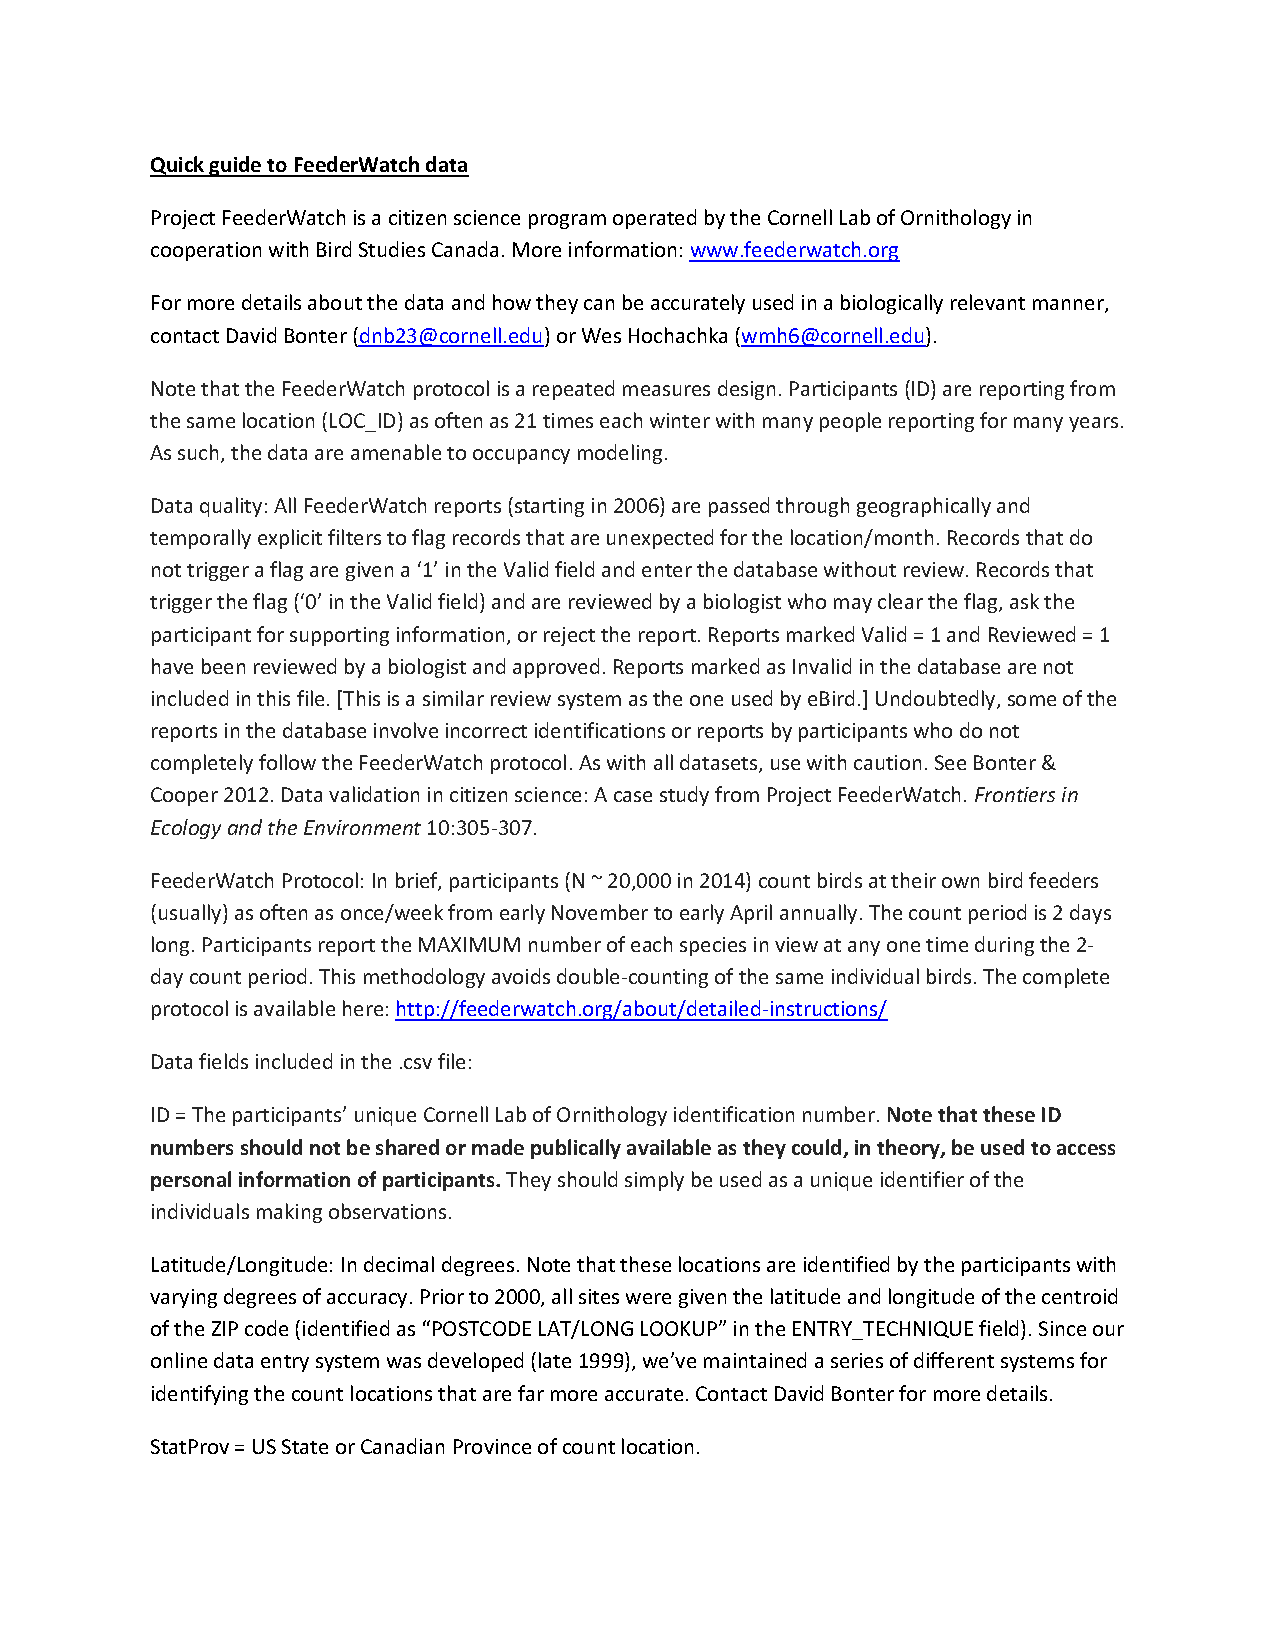
\includepdf[pages=-]{appendix/pfwGuidelines.pdf}

\chapter{SCRIPT IMPLEMENTATION USING PYTHON FOR APPENDING CITIES}


\definecolor{codegreen}{rgb}{0,0.6,0}
\definecolor{codegray}{rgb}{0.5,0.5,0.5}
\definecolor{codepurple}{rgb}{0.58,0,0.82}
\definecolor{backcolour}{rgb}{0.95,0.95,0.92}

\lstdefinestyle{mystyle}{
    backgroundcolor=\color{backcolour},   
    commentstyle=\color{codegreen},
    keywordstyle=\color{magenta},
    numberstyle=\tiny\color{codegray},
    stringstyle=\color{codepurple},
    basicstyle=\footnotesize,
    breakatwhitespace=false,         
    breaklines=true,                 
    captionpos=b,                    
    keepspaces=true,                 
    numbers=left,                    
    numbersep=5pt,                  
    showspaces=false,                
    showstringspaces=false,
    showtabs=false,                  
    tabsize=2
}
 
\lstset{style=mystyle}

\lstinputlisting[language=Python]{appendix/adding_cities.py}

\chapter{SCRIPT IMPLEMENTATION USING PYTHON FOR COLLECTING WEATHER UNDERGROUND CLIMATE DATA}

\lstinputlisting[language=Python]{appendix/adding_temp_500_0.py}

